%%%%%%%%%%%%%%%%%%%%%%%%%%%%%%%%%%%%%%%%%%%%%%%%%%%%%%%%%%%%%%%%%%%%%%%%%%%%%%%%
%2345678901234567890123456789012345678901234567890123456789012345678901234567890
%        1         2         3         4         5         6         7         8

\documentclass[letterpaper, 10 pt, conference]{ieeeconf}  % Comment this line out if you need a4paper

%\documentclass[a4paper, 10pt, conference]{ieeeconf}      % Use this line for a4 paper

\IEEEoverridecommandlockouts                             %https://www.overleaf.com/2156968253fhhpgmhwnfrt % This command is only needed if 
                                                          % you want to use the \thanks command

\overrideIEEEmargins                                      % Needed to meet printer requirements.

%In case you encounter the following error:
%Error 1010 The PDF file may be corrupt (unable to open PDF file) OR
%Error 1000 An error occurred while parsing a contents stream. Unable to analyze the PDF file.
%This is a known problem with pdfLaTeX conversion filter. The file cannot be opened with acrobat reader
%Please use one of the alternatives below to circumvent this error by uncommenting one or the other
%\pdfobjcompresslevel=0
%\pdfminorversion=4

% See the \addtolength command later in the file to balance the column lengths
% on the last page of the document

% The following packages can be found on http:\\www.ctan.org
\usepackage{graphics} % for pdf, bitmapped graphics files
\usepackage{epsfig} % for postscript graphics files
\usepackage{mathptmx} % assumes new font selection scheme installed
\usepackage{times} % assumes new font selection scheme installed
\usepackage{amsmath} % assumes amsmath package installed
\usepackage{amssymb}  % assumes amsmath package installed
\usepackage{graphicx}
\usepackage{subcaption}
\usepackage{multirow}
\usepackage{booktabs}
\usepackage{comment} % for comment command
\usepackage{soul, color} % for hl command

\title{\LARGE \bf 
Automated Quantification of Inflamed Lung Regions in Chest CT by UNet++ and SegCaps: A Comparative Analysis in COVID-19 Cases}

\author{Priya Bhatia$^{1}$, Abhishar Sinha$^{1}$, Swati Purohit Joshi$^{2}$, 
Rahuldeb Sarkar$^{3}$, Rajesh Ghosh$^4$, Soumya Jana$^{5}$  
% <-this % stops a space
%\thanks{*This work was not supported by any organization}% <-this % stops a space
%\thanks{The work was partly supported by Grant BT/PR16582/BID/7/667/2016, Department of Biotechnology (DBT), and SRM by Visvesvaraya PhD Scheme for Electronics and Information Technology, Ministry of Electronics and Information Technology (MeitY), Government of India.}
\thanks{$^{1}$Department of Artificial Intelligence, Indian Institute of Technology Hyderabad, India.}%
\thanks{$^{2}$Department of  Radiodiagnosis, Mahatma Gandhi Medical College and Hospital (MGMCH), Jaipur, India.}%
\thanks{$^{3}$Medway NHS Foundation Trust, United Kingdom.}%
\thanks{$^{4}$East Kent Hospitals University NHS Foundation Trust, United Kingdom.}%.}%
\thanks{$^{5}$Department of Electrical Engineering, Indian Institute of Technology Hyderabad, India.}%
}


%\author{ <-this % stops a space
% \thanks{}% <-this % stops a space
% \thanks{$^{1}$ Undergraduate Student, Electrical Engineering, IIT Hyderabad
%         {\tt\small ee15btech11030@iith.ac.in}}%
% \thanks{$^{2}$Undergraduate Student, Electrical Engineering, IIT Hyderabad
%         {\tt\small ee15btech11006@iith.ac.in}}%
% \thanks{$^{3}$Associate Professor, Electrical Engineering, IIT Hyderabad
%         {\tt\small ee15btech11006@iith.ac.in}}%
%}


\begin{document}



\maketitle
\thispagestyle{empty}
\pagestyle{empty}

\graphicspath{{}{images/}}
%%%%%%%%%%%%%%%%%%%%%%%%%%%%%%%%%%%%%%%%%%%%%%%%%%%%%%%%%%%%%%%%%%%%%%%%%%%%%%%%
\begin{abstract}
During the current COVID-19 pandemic, a high volume of lung imaging has been generated in the aid of the treating clinician. Importantly, lung inflammation severity, associated with the disease outcome, needs to be precisely quantified. Producing consistent and accurate reporting in high-demand scenarios can be a challenge that can compromise patient care with significant inter- or intra-observer variability in quantifying lung inflammation in a chest CT scan. In this backdrop, automated segmentation has recently been attempted using UNet++, a convolutional neural network (CNN), and results comparable to manual methods have been reported. In this paper, we hypothesize that the desired task can be performed with comparable efficiency using capsule networks with fewer parameters that make use of an advanced vector representation of information and dynamic routing. In this paper, we validate this hypothesis using SegCaps, a capsule network, by direct comparison, individual comparison with CT severity score, and comparing the relative effect on a ML(machine learning)-based prognosis model developed elsewhere. We further provide a scenario, where a combination of UNet++ and SegCaps achieves improved performance compared to individual models.



%SegCaps 


%*** In this paper, we aimed to develop an automated image segmentation algorithm to detect and quantify the inflammation in the lung with the help of CNN and Capsule Network-based models. Convolution neural network(CNNs) has shown great potential over the last few years in medical image segmentation tasks. The new architecture which was introduced by Sabour et al. called Capsule Networks with Dynamic Routing has shown great potential results for digit recognition tasks and on small image classification tasks. The reason behind the success of Capsule Networks lies in the fact that they preserve more information about the input by replacement of max-pooling layers with convolutional strides and dynamic routing. The new proposed architecture named SegCaps introduced by Rodney LaLonde and Ulas Bagci expands the use of Capsule Networks for object segmentation task, we applied the proposed SegCaps to segment infectious region inside the lungs and further compared it with CNN based model named UNet++.
%Various ophthalmic procedures critically depend on high-quality images. For instance, efficiency of teleophthalmology, a framework to bring advanced eye care to remote regions, is determined by the capability of assessing diagnostic quality of ocular fundus photographs (FPs), and rejecting poor-quality ones at the source. In this context, we study algorithmic methods of classifying high- and low-quality FPs.  Crucially, diagnostic quality (DQ) -- determined by clinically, but not necessarily perceptually, significant structures -- is not synonymous with perceptual appeal. Yet, traditional methods handpick features individually (or in small subsets) to meet certain ad hoc perceptual requirements. In contrast, we investigate the efficacy of a comprehensive set of structure-preserving features, systematically generated by a deep scattering network (ScatNet). Specifically, we consider three advanced machine learning classifiers, train each using ScatNet as well as traditional features separately, and demonstrate that the former ensure significantly superior performance for each classifier under multiple criteria including classification accuracy.
\end{abstract}
    

%\section{Introduction}
\input{intro}



%\section{Materials and Methods}
\begin{comment}
\begin{figure}[!t]
    \centering
  \begin{tabular}{cc}
    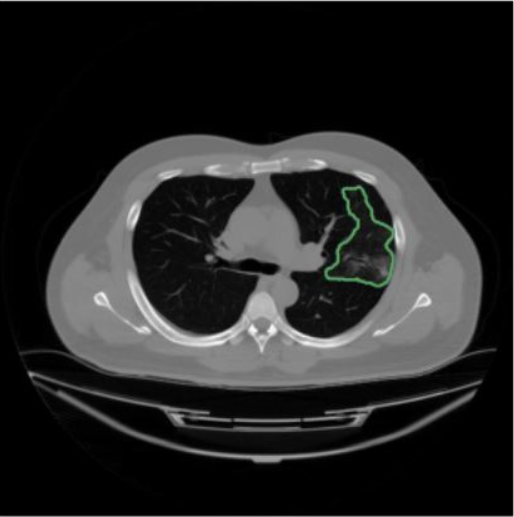
\includegraphics[width=0.45\columnwidth]{Dense_1.1.PNG} 
    &
    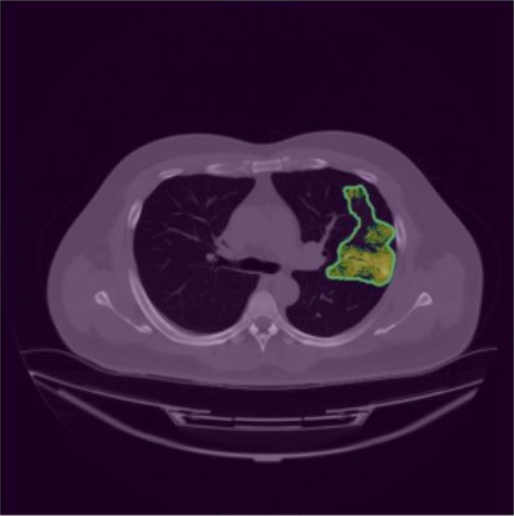
\includegraphics[width=0.45\columnwidth]{Dense_1.2.PNG} 
    \\
    (a) & (b)
    \end{tabular}
     \caption{Axial CT: inflammation mask (a) with original (expert) annotated boundary in green \cite{roth2021rapid}; (b) for (machine-identified/preprocessed) dense areas in yellow along with original boundary in green.}
     \label{Fig: Dense Masks}
\end{figure}
\end{comment}
\begin{figure*}
\centering
\begin{tabular}{c c c c}
    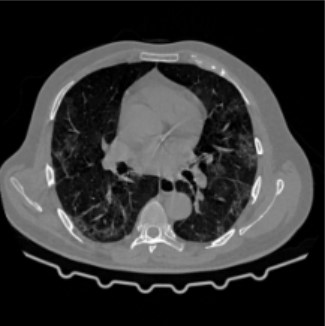
\includegraphics[scale=0.46]{Result1-30-ct.jpg} & \!\!
    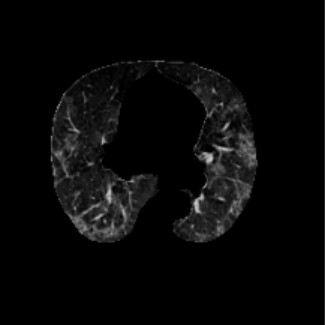
\includegraphics[scale=0.46]{images/Result1-30-extracted.jpg} & \!\!
    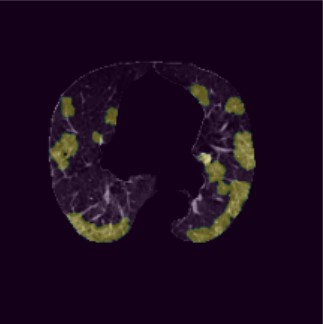
\includegraphics[scale=0.46]{images/Result1-30-unet.jpg} & \!\!
    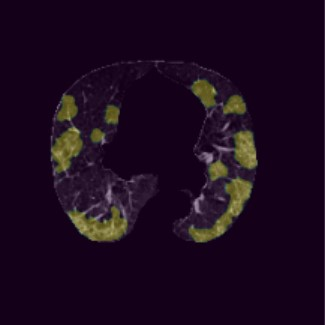
\includegraphics[scale=0.46]{images/Result1-30-capsnet.jpg}\\
    
    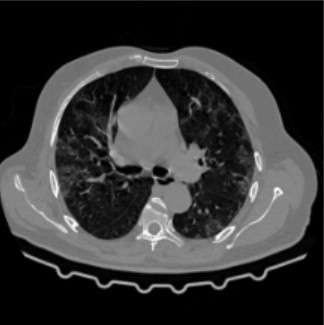
\includegraphics[scale=0.46]{images/Result2-25-ct.jpg} & \!\!
    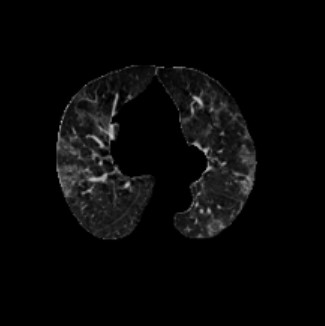
\includegraphics[scale=0.46]{images/Result2-25-extracted.jpg} & \!\!
    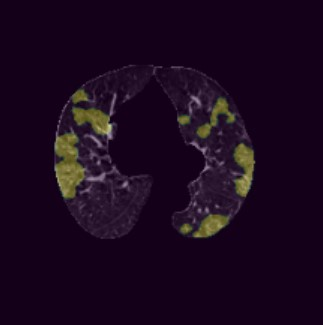
\includegraphics[scale=0.46]{images/Result2-25-unet.jpg} & \!\!
    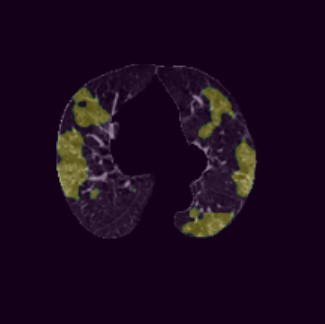
\includegraphics[scale=0.46]{images/Result2-25-capsnet.jpg}\\
    
    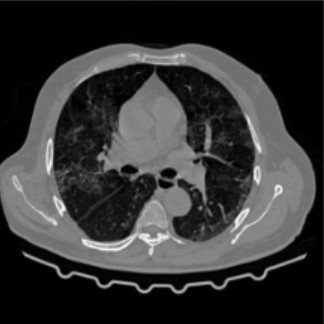
\includegraphics[scale=0.46]{images/Result3-27-ct.jpg} & \!\!
    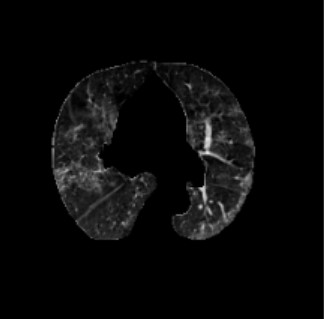
\includegraphics[scale=0.47]{images/Result3-27-extracted.jpg} & \!\!
    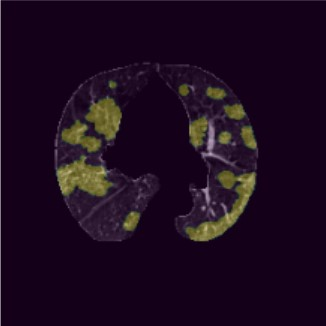
\includegraphics[scale=0.47]{images/Result3-27-unet.jpg} & \!\!
    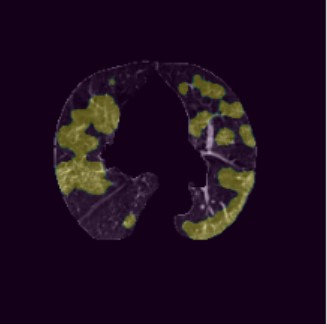
\includegraphics[scale=0.47]{images/Result3-27-capsnet.jpg}\\
    (a) & (b) & (c) & (d)
\end{tabular}
\caption{{(a)} Axial slice of CT scan; {(b)} Region Of Interest; {(c)} Inflammation Segmentation using UNet++; (d) Inflammation Segmentation using SegCaps.}
\label{Fig : Main Results}
\end{figure*}




\section{{Materials and Methods}}
\label{sec:MM}

Public datasets of chest CT scans of COVID-19 patients with annotated lung findings were used to train the deep networks UNet++ and SegCaps. A part of the study involving retrospective patient data was approved by the Institute Review Board (IRB) of Mahatma Gandhi Medical College and Hospital (MGMCH), Jaipur, India. The informed consent was waived due to the retrospective observational nature of the study and all data were anonymized before being analysed by research team, who were not part of the clinical team. All methods were performed in accordance with the relevant guidelines and regulations of the IRB of MGMCH.

\subsection{{Data Description}}
\label{sec:Data Description}
\begin{comment}
Of the COVID-19 CT Lung and Infection Segmentation Dataset \cite{jun2020covid}, we made use of a subset with 2581 non-contrast axial  CT scans (with both slice thickness and distance of 1-1.2mm) from 10 subjects for developing a lung segmentation model \cite{coronacases}.
\end{comment}
For training and testing inflammation segmentation models, we used the dataset from COVID-19 Lung CT Lesion Segmentation Challenge with 13705 non-contrast axial CT scans (with both slice thickness and distance of 5mm) from 199 subjects \cite{roth2021rapid}.
Clinical and radiological data of 302 subjects were collected at MGMCH. This dataset was used, for comparing the algorithmically quantified lung inflammation with the CT severity score manually obtained by the radiologist.
%Clinical and radiological data was collected at MGMCH between October to Decmeber 2020. This dataset was used, for comparing the algorithmically generated lung inflammation quantification with the manually calculated CT severity score by a radiologist. This dataset included CT scans as well as clinical, demographic, biochemical, and CT severity score for 302 COVID19 patients. Volumetric thin section CT scans were obtained with slices of 0.6mm each with high spatial frequency. This dataset also had missing values which was handled using data imputation. Mainly, the missing day of presentation was imputed with the median value. Remaining features which contained missing values were imputed using the nearest neighbors method with the assumption that data with similar values of known parameters may also have similar values for the unknown parameters.



\subsection{Segmentation Methods}
\label{sec:Segmentation Methods}

The task of semantically segmenting an image can be accomplished by designing a deep structure that extracts useful features using suitable arrangement of convolution operations, and summarizes such information to create a segmentation map as an output. Next, we describe UNet++ and SegCaps, the two such structures at hand.

\subsubsection{UNet++}

A predecessor CNN model, UNet, consists of encoder-decoder architecture with skip pathways connecting encoder blocks to decoder blocks. As depicted in Fig. \ref{fig:models}(a), UNet++ brings in three additions, namely, redesigned skip pathways, dense skip connections and deep supervision. These enable it to more effectively capture fine-grained details by gradually enriching high-resolution feature maps from the encoder network, and fusion with the corresponding semantically rich feature maps from the decoder network. While training this model, we performed the following augmentations: addition of Gaussian random noise with mean 0 and standard deviation 0.01, random rotations in the range -10 to 10 degrees, and random cropping to central 90\% of the image. The 1 - intersection over union (IOU loss) was minimized using was Adam optimizer with initial learning rate of $10^{-4}$.


\subsubsection{SegCaps}

In contrast to CNN models, which represent neuron-level information as scalars, capsule networks represent
such information as vectors of  spatial orientation, magnitude and other attributes. Specifically, we adopt the SegCaps architecture, consisting of various 2D convolution and deconvolution operations giving rise to 16D (16-dimensional) capsules,
and utilizing dynamic routing, as depicted in Fig. \ref{fig:models}(b). The SegCaps possesses 95.4\% fewer parameters compared to the UNet++. The same method was followed for training this models as that of UNet++ with the exception of removing rotation augmentation for this model.

%\subsection{Lung Segmentation}
%\label{sec:Lung Segmenation}



\subsection{Inflammation Segmentation}
\label{sec:Inflammation Segmenation}

Given a chest CT scan, we delineated the entire lung region by generating suitable lung mask as detailed elsewhere \cite{Sinha2022.01.30.22269998}, and used it as the region of interest (ROI). The original annotations of inflamed regions appear to often be overestimates. This can be seen in a representative case (Figs. \ref{Fig : Radiologist comparison}(a) and \ref{Fig : Radiologist comparison}(b)), where a practicing senior radiologist re-performed the annotation. Further, healthy lung areas being labeled as anomalous potentially confound ML models. To avoid this, we shrank the originally annotated region to a high-severity subregion using morphological geodesic active contour (Fig. \ref{Fig : Radiologist comparison}(c)) \cite{caselles1997geodesic}. Subsequently, we used such shrunk regions as baseline for training and testing our models. 

We measure segmentation accuracy in terms of Dice coefficient (DC) between predicted ($Y$) and baseline ($X$) inflammation regions, defined by $\mbox{DC} = {2|X\cap Y|}/{|X|+|Y|}$,
where $|X|$ indicates the area of $X$. By stacking, we also generated and quantified lung and inflammation volumes, and reported automated lesion to lung ratio (ALLR), the fraction of lung volume that is inflamed \cite{Sinha2022.01.30.22269998}.



\begin{comment}
Training segmentation models directly on the dataset resulted in poor performance in terms of dice score and one possible explanation is that the annotations for the Inflammation mask had both the regions having high and low density of abnormalities. Separating those two regions can improve the performance of the model. The dense region was computed by shrinking the annotations using morphological geodesic active contour, we used that dense region of abnormality as ground truth mask for further segmentation tasks as shown in Fig \ref{Fig: Dense Masks}.
\end{comment}

\begin{comment}
\\
    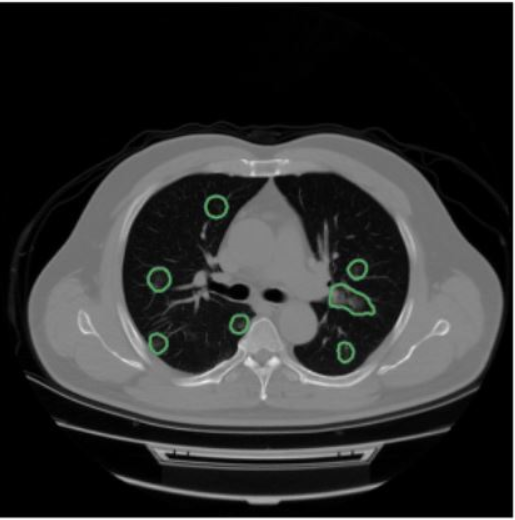
\includegraphics[width=0.45\columnwidth]{Dense_2.1.PNG} 
    &
    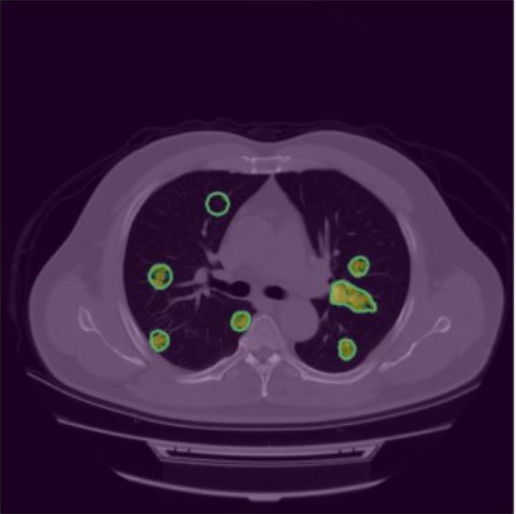
\includegraphics[width=0.45\columnwidth]{Dense_2.2.PNG} 
    \\
    (c) & (d)
\end{comment}

\begin{table}[t!]
    \centering
    \caption{Test Dice coefficient for inflammation segmentation using UNet++ and SegCaps}
    \begin{tabular}{ccc}
    \toprule 
        \textbf{Model} & \textbf{Number of epochs} & \textbf{Test Dice coefficient} \\ 
%        & \textbf{epochs} & \\
    \midrule
        UNet++ & 30 &  60\% \\
    %\hline
       SegCaps & 30 &  59.57\% \\
       \bottomrule
    %\hline 
    \end{tabular}
    \label{tab:2d-IS}
\end{table}


% UNet++ and SegCaps model were trained for binary segmentation of each of the classes.

%The following augmentations were applied to the input image and corresponding mask while training the UNet++ and SegCaps model: addition of gaussian random noise with mean 0 and standard deviation 0.01, random rotations in the range -10 to 10 degrees only in UNet++, random cropping to central 90\% of the image. The loss used was iou\_loss, and the optimizer used was Adam with initial learning rate of $10^{-4}$.

% The masks are calculated for each axial slice in a CT scan. These masks are then stacked to form a 3d Inflammation volume for a CT scan.


%as defined below:
%\begin{align*}
%\textit{ALLR} = \frac{\textit{Volume of the inflammation}}{\textit{Volume of the lung}}
%\end{align*}

% For a given CT scan first the lungs are segmented, then the inflammation region is segmented using the ROIs to calculate the ALLR. The segmentation of Inflammation region is based on the generated mask after pre-processing.

\subsection{Outcome Prediction}

Elsewhere, an ML model has been developed based on MGMCH dataset to predict an incoming COVID-19 patient's need for mechanical ventilation (MV) based on demographic, biochemical as well as the radiological parameters, and ALLR based on UNet++ and manual CT severity score have been found to perform comparably \cite{Sinha2022.01.30.22269998}. In this paper, we shall compare the performance of ALLRs based on UNet++ and SegCaps in terms of the area (AUC) under the median receiver operating characteristic (ROC) curve.


%ical as well as the radiological parameters based on the chest CT scan (if performed) along with the pre-existing conditions. For this task, we used the patient records to develop a machine learning model which predicts that whether there is a need for mechanical ventilation(MV), an acutely scarce resource, based on the MGMCH dataset. Prediction of such need is a clinically meaningful and significant outcome, which may guide efficient triaging (e.g., patients in need of MV should be admitted to a hospital in a unit where they can be monitored effectively). Now, whether patient need mechanical ventilation or not was posed as a classification task. And in order to do this task, we compared the performance with well known ensemble techniques and concluded that random forest is performing better as comparable to other models in terms of generalizability and robustness.

%The receiver operating characteristic(ROC) curve is plotted by calculating true positive rate (TPR) and false positive rate (FPR) for various threshold points of the probability generated by the model. ROC curve is convex by definition so we took the convex hull of the curve where the operating points between the optimal points are obtained by time sharing. We also calculated the area under the curve (AUC) to compare different segmentation models. It is a more useful performance metric than accuracy in cases of class imbalance, which is present in the MGMCH dataset.





%\section{Results and Discussion}



\begin{figure}[t!]
    \centering
  %\begin{subfigure}{7cm}
   % \centering
    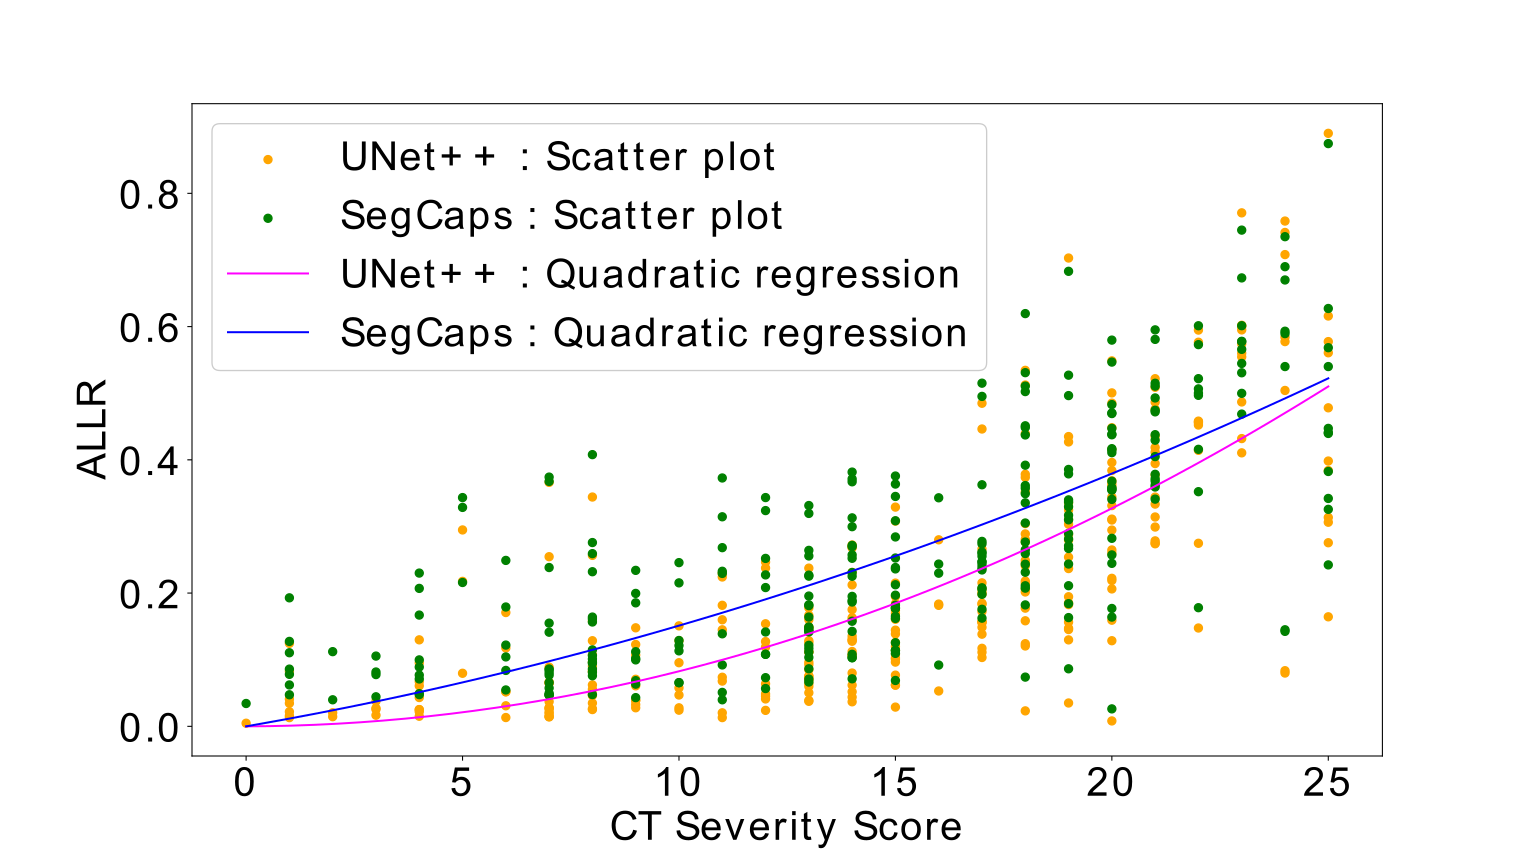
\includegraphics[width=\columnwidth]{images/Quadratic-Regression_1.png}
    %\\
     %\end{subfigure}
\caption{Scatter plots of ALLR (computed by UNet++ and SegCaps) versus CT severity score, and corresponding quadratic regression curve.}
\label{fig:RelationshipGraph}
\end{figure}

\begin{figure}[t!]
    \centering
  %\begin{subfigure}{7cm}
  %  \centering
    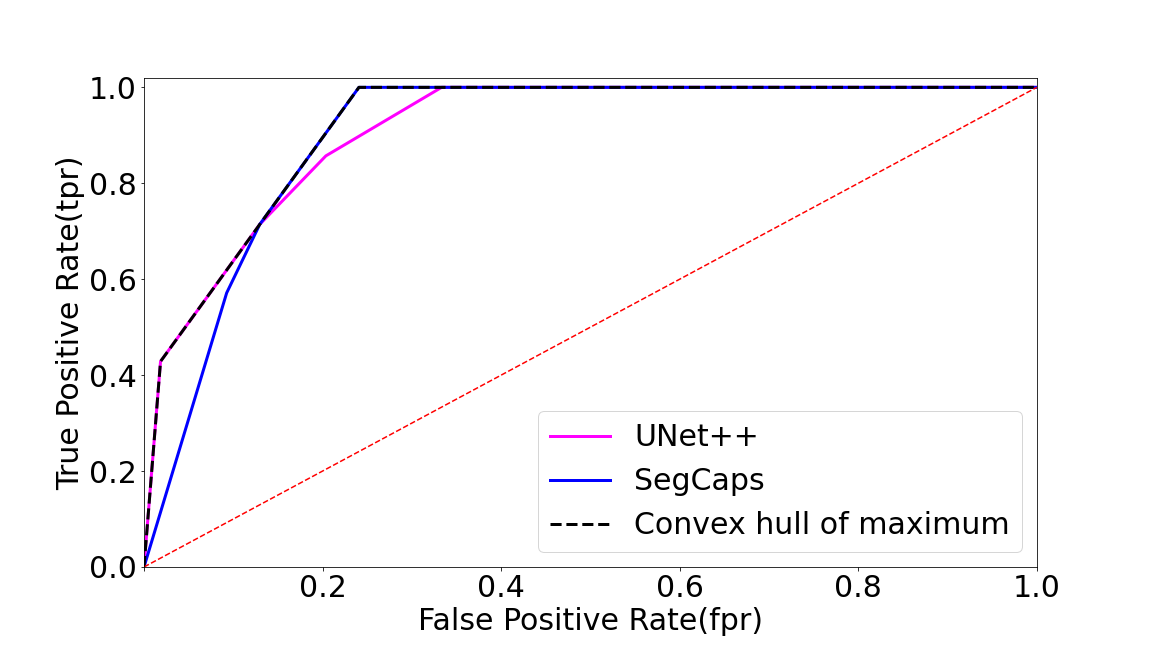
\includegraphics[width=1.0\columnwidth]{images/ROC-Overlay-fpr-tpr.png}
   % \\
% \end{subfigure}
\caption{Median ROC curves obtained by UNet++ (AUC: 0.912) and SegCaps (AUC: 0.904), as well as the convex hull of the maximum (AUC: 0.921).}
\label{fig:ROC_CUrve}
\end{figure}


\section{Experimental Results}

We begin by depicting representative CT scans, and corresponding lung segmentation and inflammation segmentation by UNet++ and SegCaps in Figs. \ref{Fig : Main Results}(a), \ref{Fig : Main Results}(b), \ref{Fig : Main Results}(c) and \ref{Fig : Main Results}(d), respectively. The results of inflammation segmentation present perceptible differences. Experts felt that UNet++ and SegCaps were slightly superior in segmenting consolidation and GGOs, respectively. However, statistically, their performances in terms of DC were nearly indistinguishable, as seen in Table \ref{tab:2d-IS}. However, this may not indicate truly similar performance, because the chosen baseline, as alluded earlier, may not provide a reliable reference.



%The segmentation performance is evaluated using multiple metrics. First, the Dice coefficient is calculated for the test subset of covid-challenge-dataset. Second, ALLRs generated for the MGMCH dataset using the segmentation models is compared with the CT severity scores. Finally,  outcome prediction models for need for ventilation in this set of patients, each using lung inflammation quantification by the three methods in question are compared. 




%Dice coefficients (DCs) for both UNet++ and SegCaps models were nearly equal. The values of DCs were relatively low, and we investigated this further. We found that there was overestimation of the inflamed area in the Covid segmentation challenge dataset when we performed in-house annotation of lung segments (by a practicing senior radiologist) as shown in Fig. \ref{Fig : Radiologist comparison}. Therefore, during our we modified the annotations and took only the region which have high density of inflammation in the mask, it cause somewhat underestimation in the generated mask and that intuition was also confirmed by the radiologists and is shown .

%Some examples of results obtained after UNet++ segmentation and SegCaps segmentation on MGMCH data are given in Fig \ref{Fig : Main Results}.

Towards more reliable comparison, scatter plot of ALLRs based on UNet++ (as well as SegCaps) versus CT severity scores is presented in Fig. \ref{fig:RelationshipGraph}. We obtained the quadratic regression curve in each case, and the respective root mean squared errors of 0.118 and 0.121 for UNet++ and SegCaps models. For linear regression, which provided a worse fit, respective correlation coefficients were 0.70 and 0.68. By these measures too, UNet++ and SegCaps performed almost similarly.

However, as shown in Fig. \ref{fig:ROC_CUrve}, the median ROC curves for predicting the need for MV using ALLRs based on UNet++ and SegCaps were found to be significantly different. Specifically, UNet++ performs superior in the low-FPR regime, and SegCaps in the high-FPR regime. This phenomenon possibly corroborates the aforementioned subjective opinion regarding their performance difference in case of consolidation and GGOs. In any case, by choosing the better tool in each regime, one may operate at a performance level (in terms of AUC) higher than either can achieve.   



% The AUC stands for "Area under the ROC Curve" shown in fig \ref{fig:ROC_CUrve} has median of 0.912 and standard deviation of 0.059 for UNet++ model and median of 0.904 and standard deviation of 0.054 in case of SegCaps. The dashed line in the curve shown in fig \ref{fig:ROC_CUrve} represents the convex hull whose combined auc median is 0.921.

\section{Discussion}

Here, we treated various types of lung parenchymal changes as the same class.
Class-wise differentiation (possibly statistically) and inflammation quantification may produce a more accurate score for the overall degree of lung inflammation, reflecting lung pathophysiology better. This work potentially opens up an area of discussion for choosing the most appropriate tool for quantification of various lung pathologies, which can be put to precise clinical use if they can be made context specific. For example, if a radiologist sees a GGO specific disease in a particular CT scan, s/he may choose to use a tool that is more appropriate for GGO while quantifying the total area involved in the disease, and use a different tool for consolidation-predominant disease. 


\bibliography{refs}
\bibliographystyle{ieeetr}
\end{document}
